\documentclass[a4paper,11pt]{article}
\usepackage[american]{babel}
\usepackage[utf8]{inputenc}
\usepackage{geometry}
\usepackage{booktabs}  
\usepackage{graphicx} 
\usepackage{listings}
\usepackage{amsmath,amsthm,amssymb}
\lstset{%
backgroundcolor=\color{cyan!10},
basicstyle=\ttfamily,
numbers=left,numberstyle=\scriptsize
}
\setlength{\parindent}{0cm}
\usepackage[wby]{callouts}

\title{Memoria Práctica 1}
\author{Álvaro Beltrán}

\begin{document}

\maketitle




\section{Búsqueda iterativa de óptimos}

\subsection{Algoritmo gradiente descendiente}


\textbf{Enunciado.} Implementar el algoritmo de gradiente descendiente \\
\textbf{Solución.} He implementado una función que hace el gradiente descendiente,en la que uso la función, su vector gradiente, un número máximo de iteraciones y un número epsilon que debe ser menor o igual que el valor de la función en los pesos. Para el criterio de parada del bucle tenemos tanto las iteraciones máximas como el epsilon.
\begin{lstlisting}
def gd(w, lr, grad_fun, fun, epsilon, max_iters = 50):		
    it=0
    while(it<max_iters and fun(w)>=epsilon):
        w_ant=np.copy(w)
        for j in range(len(w) ):
            w[j] = w[j] - lr*grad_fun(w_ant)[j]
        it+=1
    return w,it
\end{lstlisting}


\subsection{Usar GD en la función E(u,v)}
\textbf{Enunciado.} Considerar la función $E(u,v)= (ue^{v}-2ve^{-u})^{2}$. Usar Gradiente descendiente para encontrar un mínimo de esta función, comenzando desde el punto $(u,v)=(1,1)$ y usando una tasa de aprendizaje $\eta=0.1$.

\begin{enumerate}
\item[a)]Calcular analíticamente y mostrar la expresión del gradiente de la función $E(u,v)$
\item[b)]¿Cuántas iteraciones tarda el algoritmo en obtener por primera vez un valor de $E(u,v)$ inferior a $10^{-14}$?
\item[c)]¿En qué coordenadas $(u,v)$ se alcanzó por primera vez un valor igual o menor a $10^{-14}$ en el apartado anterior?
\end{enumerate}

\textbf{Solución. a)}
\begin{align*}
\nabla E(u,v)=(\partial u E(u,v),\partial v E(u,v) )= (2(ue^{v}-2ve^{-u})(e^{v}+2ve^{-u}),2(ue^{v}-2ve^{-u})(ue^{v}-2e^{-u}) )
\end{align*}

\textbf{Solución. b)} El algoritmo tarda 10 iteraciones en conseguir un valor inferior a $10^{-14}$.\\

\textbf{Solución. c)} Se alcanzó en (u,v)=( 0.04473629039778207 ,  0.023958714099141746 )\\

\textbf{Comentario} Las coordenadas obtenidas tienen sentido, pues como vemos en la figura el mínimo se alcanza cerca del cero.

\begin{figure}[h]
\includegraphics[scale=0.5]{Ejercicio1.1}
\centering
\end{figure}


\subsection{Usar GD en la función f(x,y)}
\textbf{Enunciado.} Considerar la función $f(x,y)= (x-2)^{2}+2(y+2)^{2}+2sin(2\pi x)sin(2\pi y)$.

\begin{enumerate}
\item[a)]Usar gradiente descendiente para minimizar esta función. Usar como punto inicial $(x_{0}=1,y_{0}=-1)$,(tasa de aprendizaje $\eta=0.01$ y un máximo de 50 iteraciones). Generar un gráfico de cómo desciende el valor de la función con las iteraciones. Repetir el experimento pero usando $\eta=0.1$, comentar las diferencias y su dependencia de $\eta$.
\item[b)]Obtener el valor mínimo y los valores de las variables (x,y) en donde se alcanzan cuando el punto de inicio se fija en: (2.1,-2.1),(3,-3),(1.5,1.5),(1,-1)
\end{enumerate}
\newpage
\textbf{Solución. a)}
Aquí tenemos el gráfico de como desciende al mínimo con la tasa de aprendizaje igual a 0.01 . \\

\begin{figure}[h]
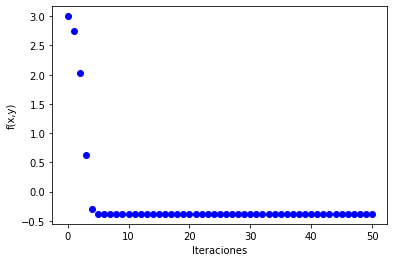
\includegraphics[scale=0.6]{grafica1ej3a}
\centering
\end{figure}

Aquí tenemos el gráfico de como desciende al mínimo con la tasa de aprendizaje igual a 0.1 .

\begin{figure}[h]
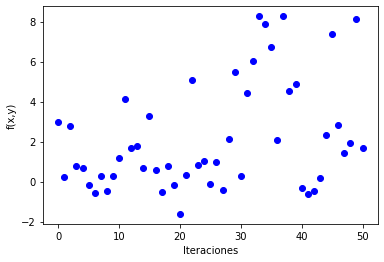
\includegraphics[scale=0.6]{grafica2ej3a}
\centering
\end{figure}

Claramente vemos una diferencia entre el primer gráfico y el segundo. En el primero vemos como desciende el valor de la función hacia el mínimo rápidamente, mientras que en el segundo gráfico en cada iteración va dando saltos debido a que hemos cogido una tasa de aprendizaje demasiado alta haciendo un efecto de rebote con las paredes opuestas de la concavidad de la gráfica de f. La tasa de aprendizaje igual a 0.01 funciona bien en esta gráfica porque para este ejemplo es un valor relativamente pequeño. \\

\newpage

\textbf{Solución. b)}


\begin{table}[h]
\begin{tabular}{|l|lll}
\hline
\multicolumn{1}{|c|}{$(x_{0},y_{0})$} & \multicolumn{1}{c|}{$\eta$} & \multicolumn{1}{c|}{(x,y)}                 & \multicolumn{1}{c|}{f(x,y)}  \\ \hline
\multicolumn{1}{|c|}{(2.1,-2.1)}      & \multicolumn{1}{c}{0.01}    & \multicolumn{1}{c}{( 2.24380 ,-2.23792 )}  & \multicolumn{1}{c}{-1.82007} \\ \cline{1-1}
\multicolumn{1}{|c|}{(3,-3)}          & \multicolumn{1}{c}{0.01}    & \multicolumn{1}{c}{( 2.73093,  -2.71327 )} & \multicolumn{1}{c}{-0.38124} \\ \cline{1-1}
\multicolumn{1}{|c|}{(1.5,1.5)}       & \multicolumn{1}{c}{0.01}    & \multicolumn{1}{c}{( 1.77792 ,  1.03205 )} & \multicolumn{1}{c}{18.0420}  \\ \cline{1-1}
\multicolumn{1}{|c|}{(1,-1)}          & 0.01                        & ( 1.26906 ,  -1.28672 )                    & \multicolumn{1}{c}{-0.38124} \\ \hline
$(x_{0},y_{0})$                       & \multicolumn{1}{l|}{$\eta$} & \multicolumn{1}{l|}{(x,y)}                 & \multicolumn{1}{l|}{f(x,y)}  \\ \hline
(2.1,-2.1)                            & 0.1                         & ( 0.13433 , -1.25353 )                     & 3.10076                      \\ \cline{1-1}
(3,-3)                                & 0.1                         & ( 2.14133 , -0.53615 )                     & 4.65511                      \\ \cline{1-1}
-0.38124                              & 0.1                         & ( 1.49926 , -2.56860 )                     & 0.90121                      \\ \cline{1-1}
(1.5,1.5)                             & 0.1                         & ( 2.66195 , -1.44300 )                     & 1.65514                      \\ \cline{1-1}
\end{tabular}
\end{table}

\subsection{Conclusión sobre el mínimo global}
\textbf{Enunciado.} ¿Cuál sería su conclusión sobre la verdadera dificultad de encontrar el mínimo global de una función arbitraria?\\

\textbf{Solución.} La dificultad se encuentra en que con el punto inicial lo que conseguimos es llegar a un mínimo local de la función desde ese punto guiandonos por la pendiente de la función cerca de ese punto. Para encontrar el mínimo global deberíamos escoger un punto lo suficiente mente cerca del mínimo global para que reiteradamente el algoritmo de gradiente descendiente nos vaya acercando hacia el mínimo.\\ 

Incluso estando lo suficientemente cerca podríamos encontrarnos problemas si tenemos mínimos relativos más cercas que este mínimo global o si llegamos a un lugar donde la pendiente es cero pero todavía no estamos en el mínimo.\\

Por último, si asumimos que somos capaces de encontrar ese punto inicial suficientemente bueno; tenemos que estudiar que tasa de aprendizaje imponer para llegar al mínimo lo suficientemente rápido sin escoger un valor demasiado grande ni demasiado pequeño.\\

Por tanto, ante una función desconocida es prácticamente imposible saber si el mínimo encontrado es local o global.


\section{Ejercicio sobre Regresión Lineal}

Este ejercicio ajusta modelos de regresión a vectores de características extraídos de imágenes de dígitos manuscritos. En particular se extraen dos características concretas: el valor medio del nivel de gris y simetría del número respecto de su eje vertical. Solo se seleccionarán para este ejercicio las imágenes de los números 1 y 5.

\subsection{Estimar modelo de RL sobre los datos proporcionados}
\textbf{Enunciado.} Estimar un modelo de regresión lineal a partir de los datos proporcionados de dichos números (Intensidad promedio, Simetría) usando tanto el algoritmo de la pseudoinversa como Gradiente descendente estocástico (SGD). Las etiquetas serán $\{-1, 1\}$, una para cada vector de cada uno de los números. Pintar las soluciones obtenidas junto con los datos usados en el ajuste. Valorar la bondad del resultado usando Ein y Eout (para Eout calcular las predicciones usando los datos del fichero de test). \\

\textbf{Solución.}\\

Algoritmo del \textsf{Gradiente descendiente estocástico} : \\

Es el mismo algoritmo que el gradiente descendiente del ejercicio 1.1, con la diferencia de que la función gradiente cogemos la coordenada j-enésimo del gradiente y evaluamos en un subconjunto del vector de características de tamaño definido escogido aleatoriamente. \\

Gráfico y recta de regresión del conjunto de datos para train:\\

\begin{figure}[h]
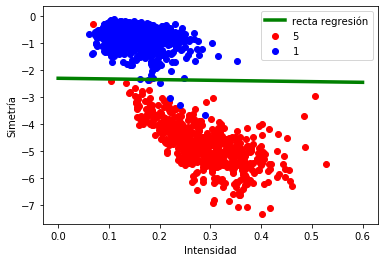
\includegraphics[scale=0.5]{grafica1ej2.1}
\centering
\end{figure}

Gráfico y recta de regresión del conjunto de datos para test:\\

\begin{figure}[h]
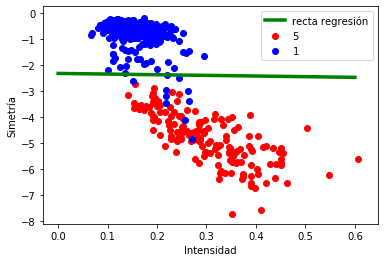
\includegraphics[scale=0.5]{grafica2ej2.1}
\centering
\end{figure}

Los errores producidos con el algoritmo Gradiente descendiente estocástico son:\\

$E_{in}$:  0.2233991068731096\\
$E_{out}$:  0.25863179195538877\\

Como vemos en los errores son errores relativamente pequeños por lo que se puede decir que el algoritmo a funcionado correctamente, con respecto a la comparativa de los errores dentro y fuera de la muestra de entrenamiento vemos que son muy parecidos por lo que el algoritmo ha conseguido abstraer bien la información a toda la población.\\

Algoritmo de la \textsf{Pseudoinversa}:
\begin{align*}
X^{\dagger}=(XX^{T})^{-1}X^{T} , w=X^{\dagger}y
\end{align*}

Gráfico y recta de regresión del conjunto de datos para train:\\

\begin{figure}[h]
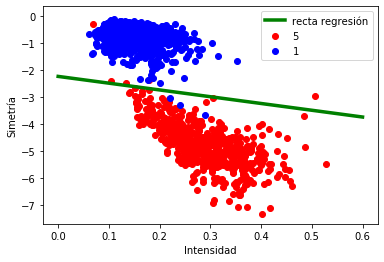
\includegraphics[scale=0.5]{grafica3ej2.1}
\centering
\end{figure}

Gráfico y recta de regresión del conjunto de datos para test:\\

\begin{figure}[h]
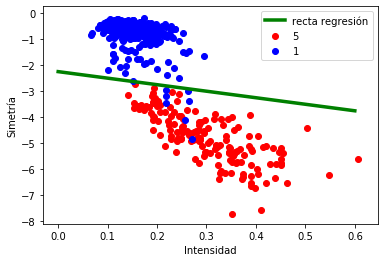
\includegraphics[scale=0.5]{grafica4ej2.1}
\centering
\end{figure}
\newpage
Los errores producidos con el algoritmo de la Pseudoinversa son:\\

$E_{in}$:  0.07918658628900384\\
$E_{out}$:  0.13095383720052572\\

Este algoritmo parece por los errores que ha funcionado mejor, pero en cuanto a la diferencia con los datos de test hay más diferencia que con el gradiente descendiente estocástico, pero sin embargo el error es menor con este algoritmo.

\subsection{Ejemplo aumentando la complejidad del modelo lineal}

\textbf{Enunciado.} En este apartado exploramos como se transforman los errores $E_{in}$ y $E_{out}$ cuando aumentamos la complejidad del modelo lineal usado. Ahora hacemos uso de la función $simula\_unif(N; 2; size)$ que nos devuelve N coordenadas 2D de puntos uniformemente muestreados dentro del cuadrado definido por $[-size, size] \times [-size, size]$.

\begin{itemize}
\item[1.] EXPERIMENTO:
\begin{enumerate}
\item[a)]Generar una muestra de entrenamiento de N = 1000 puntos en el cuadrado $\chi = [-1, 1] \times [-1, 1]$. Pintar el mapa de puntos 2D.
\item[b)]Consideremos la función $f(x_1, x_2) = sign((x_1 - 0.2)^{2} + (x_2)^{2}- 0.6)$ que usaremos para asignar una etiqueta a cada punto de la muestra anterior. Introducimos ruido sobre las etiquetas cambiando aleatoriamente el signo de un 10\% de las mismas. Pintar el mapa de etiquetas obtenido.
\item[c)]Usando como vector de características $(1, x_1, x_2)$ ajustar un modelo de regresión lineal al conjunto de datos generado y estimar los pesos w. Estimar el error de ajuste $E_{in}$ usando Gradiente Descendente Estocástico (SGD).
\item[d)]Ejecutar todo el experimento definido por (a)-(c) 1000 veces (generamos 1000 muestras diferentes) y
\begin{itemize}
\item Calcular el valor medio de los errores $E_{in}$ de las 1000 muestras.
\item Generar 1000 puntos nuevos por cada iteración y calcular con ellos el valor de $E_{out}$ en dicha iteración. Calcular el valor medio de $E_{out}$ en todas las iteraciones.
\end{itemize}
\item[e)]Valore que tan bueno considera que es el ajuste con este modelo lineal a la vista de los valores medios obtenidos de $E_{in}$ y $E_{out}$
\end{enumerate}
\item[2.] Repetir el mismo experimento anterior pero usando características no lineales. Ahora usaremos el siguiente vector de características: $\phi_2(x) = (1, x_1, x_2, x_1x_2, x_1^{2}, x_2^{2})$. Ajustar el nuevo modelo de regresión lineal y calcular el nuevo vector de pesos w. Calcular los errores promedio de $E_{in}$ y $E_{out}$.
\item[3.] A la vista de los resultados de los errores promedios $E_{in}$ y $E_{out}$ obtenidos en los dos experimentos ¿Que modelo considera que es el más adecuado? Justifique la decisión.
\end{itemize}

\textbf{Solución. 1.a)} \\
mapa de puntos 2D:
\begin{figure}[h]
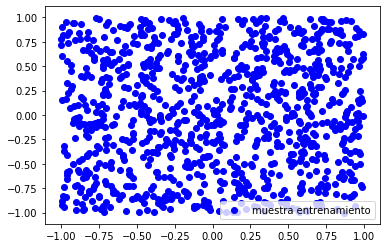
\includegraphics[scale=0.5]{grafica1ej2.21a}
\centering
\end{figure}

\textbf{Solución. 1.b)} \\
mapa de puntos etiquetados 2D:
\begin{figure}[h]
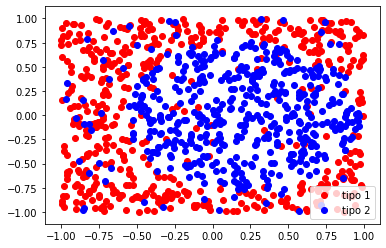
\includegraphics[scale=0.5]{grafica1ej2.21b}
\centering
\end{figure}

\textbf{Solución. 1.c)} \\
Usando grad. descendente estocástico sobre el vector de características $(1,x_1,x_2)$ conseguimos un error en la muestra de: $E_{in}$:  0.9301787342161746

Gráfico para datos train de grad. descendente estocástico junto con la recta de regresión obtenida:

\begin{figure}[h]
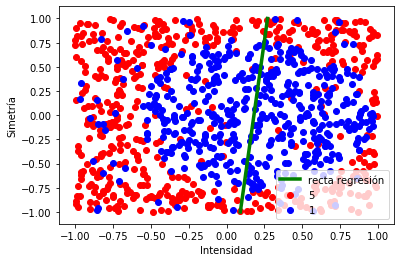
\includegraphics[scale=0.5]{grafica1ej2.21c}
\centering
\end{figure}

\textbf{Solución. 1.d)} \\
Tras mil repeticiones del experimento haciendo una media de los errores de la muestra y de la población obtenemos estos resultados:\\

$E_{in}$ media:  0.9288877657658327\\
$E_{out}$ media:  0.9347746037851759\\

\textbf{Solución. 1.e)} \\
Los errores con el modelo lineal son bastante malos, dan errores muy grandes; si es verdad que da los mismos errores dentro y fuera de la muestra, pero estos errores son demasiado malos como cabía esperar de intentar aproximar una función cuadrática con una recta.\\

\textbf{Solución. 2.}
Ahora vamos a repetir el experimento con un nuevo vector de características: $\phi_2(x) = (1, x_1, x_2, x_1x_2, x_1^{2}, x_2^{2})$. Generamos el conjunto de datos y etiquetas igual que en el apartado anterior, pero ahora usamos gradiente descendiente estocástico sobre este vector de características nuevos. Conseguimos un error en la muestra de: $E_{in}$: 0.5449312595235896.\\

Gráfico para datos train de grad. descendente estocástico junto con el conjunto obtenido:

\begin{figure}[h]
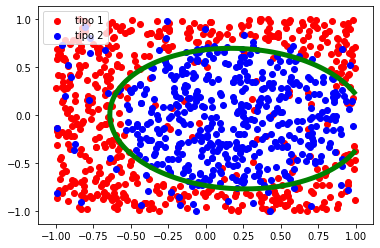
\includegraphics[scale=0.5]{grafica1ej2.22}
\centering
\end{figure}

Ahora si repetimos mil veces el experimento haciendo una media de los errores de la muestra y de la población obtenemos estos resultados:\\

$E_{in}$ media:   0.5842999458666011\\
$E_{out}$ media:  0.590928930187865\\

\textbf{Solución. 3.}
A la vista de los resultados es bastante mejor usar el vector de características $\phi_2(x) = (1, x_1, x_2, x_1x_2, x_1^{2}, x_2^{2})$, para justificar que esta sea la mejor opción tenemos una ventaja con respecto a los demás problemas y es que sabemos cual es la función que asigna las etiquetas. Si desarrollamos la expresión nos queda:
\begin{align*}
f(x_1, x_2) = sign((x_1 - 0.2)^{2} + x_2^{2}- 0.6)
=sign(x_1^{2} + 0.2^{2} - 0.4x_1 + x_2^{2}- 0.6)
\end{align*}
Como podemos ver aparecen $x_1$ y $x_2$ elevados al cuadrado, por lo que una recta ($ax+by+c=0$) no se asemeja a la expresión, mientras que una expresión cuadrática ($ax+by+cxy+dx^2+ey^2+f=0$) sí.


\section{Bonus}
\textbf{Enunciado.} Método de Newton Implementar el algoritmo de minimización de Newton
y aplicarlo a la función f(x, y) dada en el ejercicio.3. Desarrolle los mismos experimentos usando los mismos puntos de inicio.

\begin{itemize}
\item Generar un gráfico de como desciende el valor de la función con las iteraciones.
\item Extraer conclusiones sobre las conductas de los algoritmos comparando la curva de decrecimiento de la función calculada en el apartado anterior y la correspondiente obtenida con gradiente descendente.
\end{itemize}

\textbf{Solución.}
Denoto la matriz H como la matriz Hessiana ($\nabla^2f(x,y)$). Y realizo el algoritmo de Newton proporcionado en las diapositivas:
\begin{align*}
H^{\dagger}=(HH^{T})^{-1}H^{T} \\ \triangle w=-H^{\dagger}\nabla f(x,y) \\
w=w+\triangle w
\end{align*}
Usando como punto inicial $(-1,1)$ el algoritmo me encuentra un máximo local:
\begin{figure}[h]
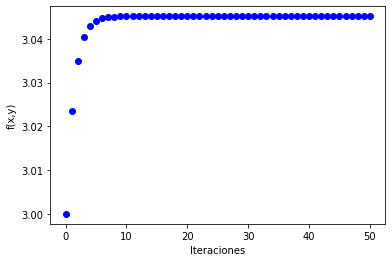
\includegraphics[scale=0.5]{bonus}
\centering
\end{figure}









\end{document}
